\chapter{Ataques}

A criptografia quântica é um campo que se encontra ainda em desenvolvimento e, como tal, está sujeito a vários tipos de ataques que podem comprometer a segurança dos sistemas de distribuição de chaves quânticas (QKD). Esses ataques podem ser amplamente classificados em duas categorias: ataques no canal quântico e ataques no canal clássico.

\section{Tipos de Ataques}

\subsection{Ataques no Canal Quântico}

Os ataques ao canal quântico visam a transmissão de estados quânticos pelo canal e podem assumir várias formas. Por exemplo, um invasor pode tentar interceptar e medir os estados quânticos para obter informações sobre a chave secreta. Isso é conhecido como ataque de intercepção e medição, e é um tipo de ataque man-in-the-middle.

Outro tipo de ataque no canal quântico é um ataque de divisão do número de fotões, no qual o atacante divide os fotões no estado quântico e mede cada metade separadamente. Isso permite que o invasor obtenha informações parciais sobre a chave secreta sem ser detectado pelas partes legítimas.

\subsection{Ataques no Canal Clássico}

Os ataques no canal clássico visam a transmissão de informações clássicas pelo canal, como mensagens de autenticação ou informações de correção de erros. Esses ataques podem assumir várias formas, como ataques de personificação, nos quais o invasor finge ser uma das partes legítimas para obter acesso à chave secreta.

Outro tipo de ataque ao canal clássico é o ataque man-in-the-middle, no qual o invasor intercepta a informação clássica e a modifica para obter acesso à chave secreta. Esse tipo de ataque pode ser difícil de detectar, pois o invasor pode manipular as informações clássicas de forma que pareçam válidas para as partes legítimas.

\begin{figure}[!hbt]
  \centering
  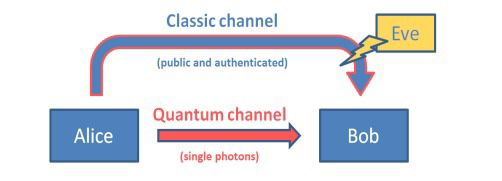
\includegraphics[width=\textwidth]{images/possible-attack.jpg}
  \caption{Figura ilustrativa de um ataque ao canal clássico.}
  \label{fig:classic-attack}
\end{figure}
\FloatBarrier

\section{Ataques Conhecidos}

Existem vários métodos conhecidos de ataque em criptografia quântica, que visam vários aspectos dos sistemas QKD. Esses métodos incluem:

\begin{itemize}
  \item Ataques de intercepção e medição, nos quais o invasor intercepta e mede os estados quânticos para obter informações sobre a chave secreta.
  \item Ataques de divisão do número de fotões, nos quais o atacante divide os fotões no estado quântico e mede cada metade separadamente.
  \item Ataques de personificação, nos quais o invasor finge ser uma das partes legítimas para obter acesso à chave secreta.
  \item Ataques man-in-the-middle, em que o invasor intercepta e modifica informações clássicas para obter acesso à chave secreta.
  \item Ataques de canal lateral, nos quais o invasor usa informações obtidas por meio de canais laterais, como perda de fotões no canal quântico, para obter informações sobre a chave secreta.
\end{itemize}

\subsection{Ataques de Intercepção e Medição}

Um ataque de intercepção e medição é um tipo de ataque em criptografia quântica que visa a transmissão de estados quânticos pelo canal. Num ataque de intercepção e medição, o invasor intercepta os estados quânticos e os mede para obter informações sobre a chave secreta.

Esse tipo de ataque é uma forma de ataque man-in-the-middle, pois o invasor é capaz de manipular a comunicação entre as partes legítimas sem ser detectado. Como o invasor está medindo os estados quânticos, ele pode obter informações parciais sobre a chave secreta sem ser detectado pelas partes legítimas.

Existem vários métodos conhecidos de detecção e mitigação de ataques de intercepção e medição. Por exemplo, códigos de correção de erros quânticos podem ser usados para detectar e corrigir erros nos estados quânticos, como perda de fotões ou erros de fase. Além disso, a autenticação quântica pode ser usada para verificar a identidade das partes envolvidas no sistema QKD e evitar ataques de representação.

\subsection{Ataques de Divisão do Número de Fotões}

Um ataque de divisão de número de fotões é um tipo de ataque em criptografia quântica que visa a transmissão de estados quânticos pelo canal. Num ataque de divisão do número de fotões, o atacante divide os fotões no estado quântico e mede cada metade separadamente. Isso permite que o invasor obtenha informações parciais sobre a chave secreta sem ser detectado pelas partes legítimas.

Os ataques de divisão do número de fotões são uma preocupação particular em sistemas QKD que usam estados coerentes fracos, pois esses estados são compostos de uma superposição de diferentes números de fotões. O atacante pode dividir o estado em duas partes, cada uma contendo um número diferente de fotões, e medir cada parte separadamente. Isso permite que o invasor obtenha informações parciais sobre a chave secreta, sem ser detectado pelas partes legítimas.

Existem vários métodos conhecidos de detecção e mitigação de ataques de divisão do número de fotões. Por exemplo, códigos de correção de erros quânticos podem ser usados para detectar e corrigir erros nos estados quânticos, como perda de fotões ou erros de fase. Além disso, a autenticação quântica pode ser usada para verificar a identidade das partes envolvidas no sistema QKD e evitar ataques de representação.

\begin{figure}[!hbt]
  \centering
  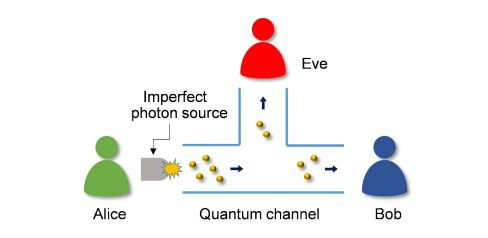
\includegraphics[width=\textwidth]{images/foton-division-attack.jpg}
  \caption{Figura ilustrativa de um ataque de divisão do número de fotões. O atacante divide o estado quântico em duas partes, cada uma contendo um número diferente de fotões. O atacante mede cada parte separadamente para obter informações parciais sobre a chave secreta.}
  \label{fig:foton-division-attack}
\end{figure}
\FloatBarrier

\subsection{Ataques de Personificação}

Um ataque de personificação é um tipo de ataque em criptografia quântica que tem como alvo as informações clássicas transmitidas pelo canal. Num ataque de personificação, o invasor finge ser uma das partes legítimas para obter acesso à chave secreta.

Esse tipo de ataque pode ser difícil de detectar, pois o invasor pode manipular as informações clássicas de forma que pareçam válidas para as partes legítimas. Por exemplo, o invasor pode usar uma identidade falsa para se autenticar para a outra parte ou pode modificar as mensagens de autenticação para obter acesso à chave secreta.

Existem vários métodos conhecidos de detecção e mitigação de ataques de personificação. Por exemplo, a autenticação quântica pode ser usada para verificar a identidade das partes envolvidas no sistema QKD e evitar ataques de personificação. Além disso, protocolos criptográficos, como protocolos de autenticação ou protocolos de troca de chaves, podem ser usados para fornecer segurança adicional e proteção contra ataques no canal clássico.

\subsection{Ataques de Canal Lateral}

Um ataque de canal lateral é um tipo de ataque em criptografia quântica que usa informações obtidas por meio de canais laterais, como perda de fotões no canal quântico, para obter informações sobre a chave secreta.

Os ataques de canal lateral podem ser difíceis de detectar, pois o invasor não manipula diretamente os estados quânticos ou as informações clássicas transmitidas pelo canal. Em vez disso, o invasor usa as informações obtidas por meio do canal lateral, como o tempo ou a intensidade dos fotões, para obter informações parciais sobre a chave secreta.

Existem vários métodos conhecidos de detecção e mitigação de ataques de canal lateral. Por exemplo, códigos de correção de erros quânticos podem ser usados para detectar e corrigir erros nos estados quânticos, como perda de fotões ou erros de fase. Além disso, os códigos clássicos de correção de erros podem ser usados para detectar e corrigir erros nas informações clássicas transmitidas pelo canal, como mensagens de autenticação ou informações de correção de erros.

\section{Métodos de defesa e mitigação conhecidos}

Embora os ataques na criptografia quântica sejam uma ameaça significativa à segurança dos sistemas QKD, também existem vários métodos conhecidos de defesa e mitigação que podem ser usados para proteger contra esses ataques. Esses métodos incluem:

\begin{itemize}
  \item Códigos de correção de erros quânticos, que podem ser usados para detectar e corrigir erros nos estados quânticos, como perda de fotões ou erros de fase.
  \item Autenticação quântica, que pode ser usada para verificar a identidade das partes envolvidas no sistema QKD e evitar ataques de personificação.
  \item Protocolos de acordo de chave quântica, que podem ser usados para estabelecer uma chave secreta compartilhada entre as partes de forma segura e autenticada.
  \item Códigos de correção de erros clássicos, que podem ser usados para detectar e corrigir erros nas informações clássicas transmitidas pelo canal, como mensagens de autenticação ou informações de correção de erros.
  \item Protocolos criptográficos, como protocolos de autenticação ou protocolos de troca de chaves, que podem ser usados para fornecer segurança adicional e proteção contra ataques no canal clássico.
\end{itemize}

\subsection{Códigos de correção de erros quânticos}

Os códigos de correção de erros quânticos são um componente chave de muitos sistemas QKD e desempenham um papel crítico na detecção e correção de erros nos estados quânticos transmitidos.

Os códigos de correção de erros quânticos são baseados nos princípios da mecânica quântica e usam estados quânticos emaranhados para codificar e transmitir as informações. Isso permite que os estados quânticos sejam protegidos contra erros, como perda de fotões ou erros de fase, que podem ocorrer durante a transmissão.

Existem vários tipos diferentes de códigos de correção de erros quânticos, que usam diferentes esquemas de codificação e oferecem diferentes níveis de proteção contra erros. Por exemplo, alguns códigos são projetados para proteger contra a perda de um único fotão, enquanto outros são projetados para proteger contra a perda de múltiplos fotões.

\subsection{Autenticação quântica}

A autenticação quântica é uma técnica utilizada em sistemas QKD para verificar a identidade das partes envolvidas na comunicação.

A autenticação quântica é baseada nos princípios da mecânica quântica e usa estados quânticos emaranhados para codificar e transmitir as informações de autenticação. Isso permite que as informações de autenticação sejam protegidas contra ataques, como ataques de personificação ou man-in-the-middle, que podem tentar obter acesso à chave secreta.

Existem vários métodos diferentes de autenticação quântica, que usam diferentes esquemas de codificação e oferecem diferentes níveis de proteção contra ataques. Por exemplo, alguns métodos usam protocolos de acordo de chave quântica para estabelecer uma chave secreta compartilhada de maneira segura e autenticada, enquanto outros usam primitivas criptográficas quânticas, como assinaturas quânticas ou compromissos quânticos, para fornecer segurança adicional.

\subsection{Protocolos de acordo de chave quântica}

Os protocolos de acordo de chave quântica são uma classe de protocolos criptográficos projetados para estabelecer uma chave secreta compartilhada entre duas ou mais partes de maneira segura e autenticada.

Esses protocolos são baseados nos princípios da mecânica quântica e usam estados quânticos emaranhados para codificar e transmitir as informações de acordo de chave. Isso permite que as informações do acordo de chave sejam protegidas contra ataques, como ataques man-in-the-middle, que podem tentar obter acesso à chave secreta.

Existem vários protocolos diferentes de acordo de chave quântica, que usam diferentes esquemas de codificação e oferecem diferentes níveis de segurança e desempenho. Por exemplo, alguns protocolos são baseados nos princípios de distribuição de chave quântica (QKD), enquanto outros são baseados nos princípios de acordo de chave quântica (QKA).

\subsection{Códigos de correção de erros clássicos}

Os códigos clássicos de correção de erros são um componente chave de muitos sistemas QKD e desempenham um papel crítico na detecção e correção de erros nas informações clássicas transmitidas.

Os códigos clássicos de correção de erros são baseados nos princípios da teoria clássica da informação e usam algoritmos matemáticos para codificar e transmitir as informações. Isso permite que as informações sejam protegidas contra erros, como erros de transmissão ou interferência, que podem ocorrer durante a transmissão.

Existem vários tipos diferentes de códigos clássicos de correção de erros, que usam diferentes esquemas de codificação e oferecem diferentes níveis de proteção contra erros. Por exemplo, alguns códigos são projetados para proteger contra erros de bit único, enquanto outros são projetados para proteger contra erros de vários bits.

\subsection{Protocolos criptográficos}

Os protocolos criptográficos são uma classe de algoritmos usados para fornecer segurança e proteção em sistemas de comunicação. Esses protocolos são baseados nos princípios da criptografia e usam técnicas matemáticas, como criptografia e autenticação, para proteger as informações transmitidas pelo canal.

Os protocolos criptográficos são um componente importante de muitos sistemas QKD e fornecem segurança e proteção adicionais contra ataques no canal clássico. Por exemplo, os protocolos de autenticação podem ser usados para verificar a identidade das partes envolvidas na comunicação e para evitar a representação ou ataques man-in-the-middle. Além disso, os protocolos de troca de chaves podem ser usados para estabelecer uma chave secreta compartilhada de maneira segura e autenticada.

Existem vários protocolos criptográficos diferentes habitualmente usados em sistemas QKD, incluindo protocolos de autenticação, protocolos de troca de chaves e primitivas criptográficas, como assinaturas ou compromissos.

\newpage
